\section{Практическая часть}

Для написания програмы основным языком был выбран Java, поскольку в данном курсе мы параллельно изучаем этот язык и написание данной программы
является хорошей практикой для его изучения.

\subsection{Как пользоваться программой}

Для парсинга аргументов командной строки используется внешняя библиотека JCommander, чтобы упростить работу,
не относящуюся непосредственно к ЭЦП.

Запускаем jar-файл с параметром \m{-h}, чтобы вызвать меню помощи:
\begin{figure}[h!]
  \center{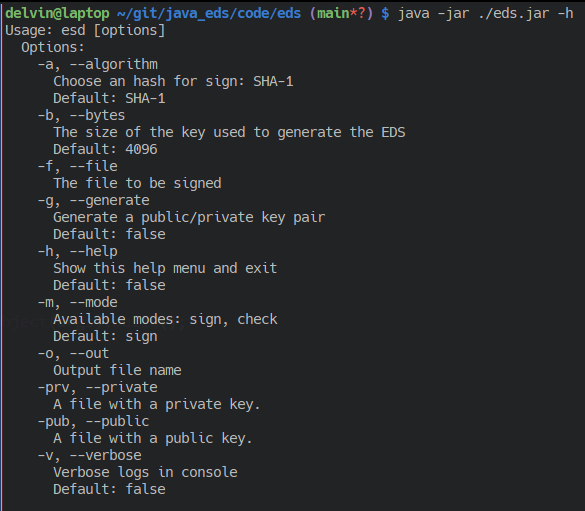
\includegraphics[scale=0.9]{img/program_usage}}
  \caption{Меню помощи}
\end{figure}

\subsubsection{Алгоритм}
Ключ \m{-a} отвечает за алгоритм хэш-функции. Программа написана с использованием интерфейсов, чтобы максимально упростить задачу добавления новых хэш-функций.
Как видно из рисунка выше, для данной работы был реализован только SHA-1, который является опцией по-умолчанию, поэтому этот параметр можно не указывать.

\subsubsection{Размер ключа}
Ключ \m{-b} отвечает за размер модуля, который будет генерироваться для алгоритма RSA.

\subsubsection{Генерация ключей}
Ключ \m{-g} отвечает за генерацию открытого и закрытого ключей ЭЦП.

\subsubsection{Файлы}
Ключ \m{-f} отвечает за файл, который необходимо подписать. Ключ '-o' - за файл, куда записать данные.

\subsubsection{Режимы работы}
Ключ \m{-m} отвечает за режим работы программы. По-умолчанию программа будет подписывать файл, если нам необходимо проверить подпись, то нужно передать параметр 'check'.

\subsubsection{Чтение ключей из файлов}
Ключ \m{-prv} указывает откуда читать данные для приватного ключа.

Ключ \m{-pub} указывает откуда читать данные для публичного ключа.

\subsubsection{Подробный режим}
Ключ \m{-v} говорит программе, что необходимо подробно описывать ход своей работы.

\newpage
\subsection{Примеры использования программы}

\begin{figure}[h!]
  \center{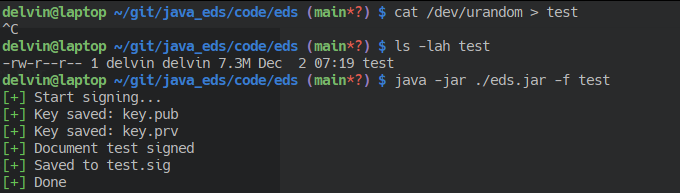
\includegraphics[scale=0.9]{img/simple_sign.png}}
  \caption{Подпись файла}
\end{figure}

\begin{figure}[h!]
  \center{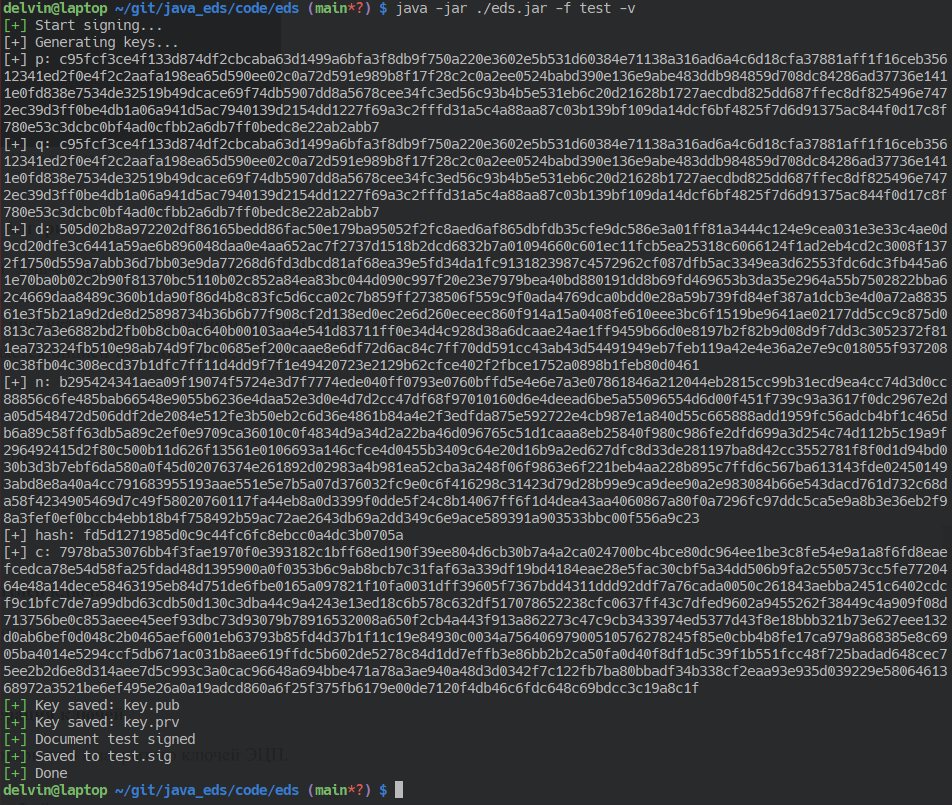
\includegraphics[scale=0.7]{img/simple_sign_verbose.png}}
  \caption{Подпись файла в подробном режиме}
\end{figure}

Как можно видеть на рисунках выше, создаётся два файла с публичным и приватным ключом. Помимо этого, в файл записывается определенная структура, которая говорит, что документ был подписан. О ней читатель узнает позже.

\begin{figure}[h!]
  \center{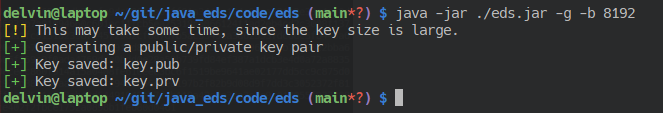
\includegraphics[scale=0.8]{img/key_gen.png}}
  \caption{Генерация ключей}
\end{figure}

\begin{figure}[h!]
  \center{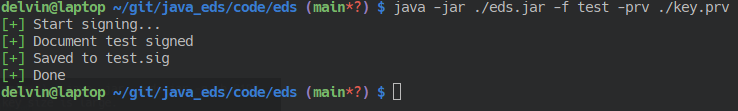
\includegraphics[scale=0.8]{img/use_key_sign.png}}
  \caption{Использование сгенерированных ключей для подписи}
\end{figure}

\begin{figure}[h!]
  \center{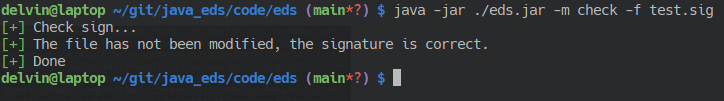
\includegraphics[scale=0.8]{img/base_check_sign.png}}
  \caption{<<Честная>> проверка подписи}
\end{figure}

\clearpage
\newpage
\subsection{Описание програмной реализации}

\subsubsection{Структура ЭЦП}
Поскольку в техническом задании не оговаривалось в каком формате необходимо хранить подпись, то мной была разработана следующая структура
пакета, которая записывается в конец файла к изначальному и позволяет хранить все необходимые данные.

Структура подписи имеет следующий вид:
\begin{table}[h!]
  \centering
  \begin{tabular}{|c|c|l|}
    \hline 
    Byte & Сообщение & Описание\\ \hline
    0 & 0xCAFEBABE & Метка, означающая начало подписи в файле \\ \hline
    4 & LEN & Размер пакета, с подписью \\ \hline
    8 & N\_LEN & Размер модуля \\ \hline 
    12 & N & Модуль публичного ключа \\ \hline
    12 + N\_LEN & E & Публичная экспонента \\ \hline
    16 + N\_LEN & C & Подписанный хэш \\ \hline
    16 + N\_LEN + len(c) & 0xCAFEBABE & Метка, означающая конец подписи \\ \hline
  \end{tabular}
\end{table}

Структура публичного ключа:
\begin{table}[h!]
  \centering
  \begin{tabular}{|c|c|l|}
    \hline 
    Byte & Сообщение & Описание\\ \hline
    0 & N\_LEN & Размер модуля \\ \hline 
    4 & N & Модуль публичного ключа \\ \hline
    4 + N\_LEN & E & Публичная экспонента \\ \hline
  \end{tabular}
\end{table}

Структура приватного ключа:
\begin{table}[h!]
  \centering
  \begin{tabular}{|c|c|l|}
    \hline 
    Byte & Сообщение & Описание\\ \hline
    0 & N\_LEN & Размер модуля \\ \hline 
    4 & N & Модуль публичного ключа \\ \hline
    4 + N\_LEN & D & Приватная экспонента \\ \hline
  \end{tabular}
\end{table}

\subsubsection{RSA}

Для реализации криптоалгоритма RSA были созданы дополнительные классы \m{PublicKey} и \m{PrivateKey}, которые
отвечают за обработку и создание соответствующих ключей.

Рассмотрим файл \m{RSA.java}, который является основным для данного алгоритма:
\begin{lstlisting}[language=Java]
public class RSA {
    private PrivateKey privateKey;
    private PublicKey publicKey;
    private Hash hash;
    private boolean verbose;

    public RSA(String hash, PrivateKey privateKey) throws NoImplementedAlgorithmException {
        this.publicKey = new PublicKey(privateKey);
        this.privateKey = privateKey;
        this.hash = MessageDigest.getInstance(hash);
    }

    public RSA(String hash, Integer keySize, boolean verbose) throws NoImplementedAlgorithmException {
        this.hash = MessageDigest.getInstance(hash);
        this.verbose = verbose;

        if (this.verbose)
            Printer.info("Generating keys...");
        this.privateKey = new PrivateKey(keySize / 2, verbose);
        this.publicKey = new PublicKey(privateKey);
    }

    public RSA(PublicKey publicKey) {
        this.publicKey = publicKey;
    }

    public byte[] encrypt(byte[] content) {
        BigInteger message = new BigInteger(1, this.hash.digest(content));

        if (this.verbose)
            Printer.info("hash: " + message.toString(16));

        // RSA signature algorithm
        BigInteger c = message.modPow(privateKey.getPrivateExponent(), privateKey.getModulo());
        if (this.verbose)
            Printer.info("c: " + c.toString(16));

        return this.getDump(c);
    }
    // ...
    public BigInteger decrypt(BigInteger signature, boolean verbose) {
        BigInteger res = signature.modPow(publicKey.getExponent(), publicKey.getModulo());
        if (verbose)
            Printer.info("Decrypted string: " + res.toString(16));
        return res;
    }
}
\end{lstlisting}

Функции \m{encrypt} и \m{decrypt} используют алгоритм \m{RSA}, описанный в теоретической части.

\subsubsection{SHA-1}

Для реализации хэш-функции был создан дополнительный интерфейс \m{Hash}, который позволяет лего добавлять реализацию хэш-функций
с использованием порождающего паттерна <<Фабричный метод>>.

Код, реализующий хэш-функцию SHA-1. Написан с опорой на спецификацию RFC\cite{SHA1Specs}.
\begin{lstlisting}[language=Java]
public class SHA1 implements Hash {
    private int h0 = 0x67452301;
    private int h1 = 0xEFCDAB89;
    private int h2 = 0x98BADCFE;
    private int h3 = 0x10325476;
    private int h4 = 0xC3D2E1F0;

    public byte[] digest(byte[] content) {
        // Create array that will store 16-word blocks
        int[] blocks = new int[(((content.length + 8) >> 6) + 1) * 16];

        for (int i = 0; i < content.length; i++)
            blocks[i >> 2] |= (content[i] & 0xff) << (24 - (i % 4) * 8);
          
        // Append padding bits like in specification
        // 0x80 == 0b10000000
        blocks[content.length >> 2] |= 0x80 << (24 - (content.length % 4) * 8);
        // Last block contains size of content
        blocks[blocks.length - 1] = content.length * 8;

        // SHA1 algorithm
        int[] w = new int[80];
        for (int i = 0; i < blocks.length; i += 16) {
            int a = h0;
            int b = h1;
            int c = h2;
            int d = h3;
            int e = h4;

            for (int j = 0; j < 80; j++) {
                if (j < 16)
                    w[j] = blocks[i + j];
                else
                    w[j] = rol(w[j - 3] ^ w[j - 8] ^ w[j - 14] ^ w[j - 16], 1);

                int f;
                int k;
                if (j < 20) {
                    f = (b & c) | ((~b) & d);
                    k = 0x5A827999;
                } else if (j < 40) {
                    f = b ^ c ^ d;
                    k = 0x6ED9EBA1;
                } else if (j < 60) {
                    f = (b & c) | (b & d) | (c & d);
                    k = 0x8F1BBCDC;
                } else {
                    f = b ^ c ^ d;
                    k = 0xCA62C1D6;
                }
                int tmp = rol(a, 5) + f + e + k + w[j];
                e = d;
                d = c;
                c = rol(b, 30);
                b = a;
                a = tmp;
            }
            h0 += a;
            h1 += b;
            h2 += c;
            h3 += d;
            h4 += e;
        }

        byte[] digest = new byte[20];
        int2b(h0, digest, 0);
        int2b(h1, digest, 4);
        int2b(h2, digest, 8);
        int2b(h3, digest, 12);
        int2b(h4, digest, 16);
        return digest;
    }
    // ...

    // Bitwise rotate 32 bit to the left
    private int rol(int num, int cnt) {
        return (num << cnt) | (num >>> (32 - cnt));
    }
} 
\end{lstlisting}

Рассмотрим, следующий кусок кода:
\begin{lstlisting}[language=Java]
for (int i = 0; i < content.length; i++)
    blocks[i >> 2] |= (content[i] & 0xff) << (24 - (i % 4) * 8);
\end{lstlisting}

Поскольку на вход программы поступает тип данных \m{byte}, а мы хотим работать с целочисленным типом данных,
то необходимо осуществить преобразование данных. Ниже приведен пример работы кода:
\begin{verbatim}
Indexes: 0, 1, 2, 3 >> 2 == 0
content[0] = 0x11
content[1] = 0x22
content[2] = 0x33
content[3] = 0x44
i == 1: 0x11000000
i == 2: 0x11220000
i == 3: 0x11223300
i == 4: 0x11223344
\end{verbatim}

Таким образом 4 байта конвертируются в целочисленное значение.

\subsubsection{Проверка на устойчивость}

Создадим простую презентацию, которую необходимо будет подписать и проверить.
Заменим несколько байт в подписанном файле, чтобы убедиться, что документ действительно был изменён и запустим программу.

\begin{figure}[h!]
  \center{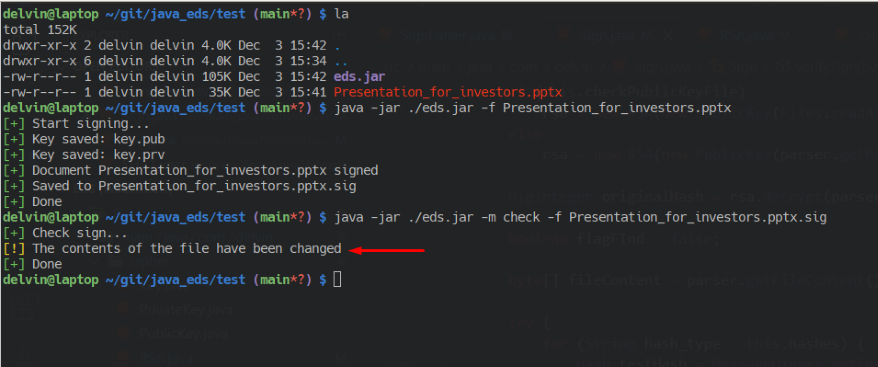
\includegraphics[scale=0.7]{img/modified_sign_program_output.png}}
  \caption{Вывод программы}
\end{figure}

\begin{figure}[h!]
  \center{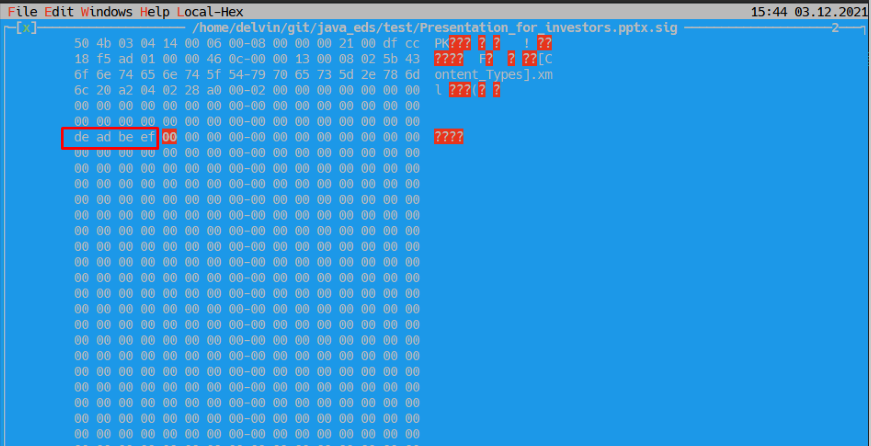
\includegraphics[scale=0.7]{img/modified_sign.png}}
  \caption{Измененные байты}
\end{figure}

Как видно на Рисунке 9 программа определяет подмену документа, даже при малейшем изменении. Это достигается благодаря лавинному эффекту 
в хэш-функции SHA-1.

\subsubsection{Анализ реальной ЭЦП}

Проведём небольшой анализ реальной ЭЦП на примере справки об обучении в образовательной организации, которую выдавал учебный отдел в
начале 2021 учебного года. Посмотрим на структуру файла.

\begin{figure}[h!]
  \center{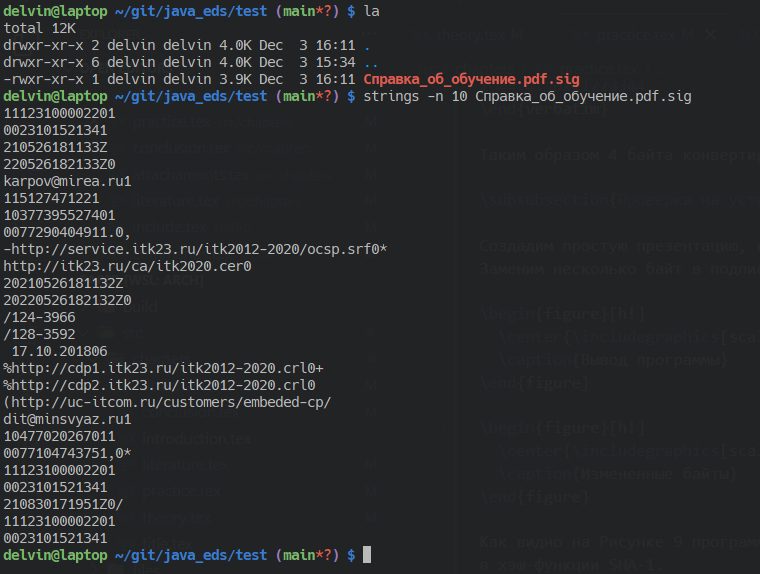
\includegraphics[scale=0.7]{img/real_sig.png}}
  \caption{ЭЦП справки}
\end{figure}

Файл оканчивается на \m{.pdf.sig}, что означает, что перед нами подпись оригинального файла. Вместо добавления данных к концу документа,
создаётся отдельный файл, который можно проверить отдельно. Это решение является правильным, поскольку не повреждает исходный файл, но по техническому заданию
требуется добавление подписи к концу файла.

Запустим утилиту \m{strings} из набора \m{binutils}, чтобы посмотреть на строки в файле. Видно, что помимо мусорных данных есть и осмысленные.

Например, \m{karpov@mirea.ru} - вероятно, почта человека, который подписывал данный документ.

Ссылка \url{http://service.itk23.ru/itk2012-2020/ocsp.srf} ведёт на файл, который содержит 5 байт информации. По имени файла \m{oscp.srf} 
можно найти, что это ничто иное как \m{Online Certificate Status Protocol}.

\emph{Протокол состояния сетевого сертификата (OCSP)} - это интернет-протокол, используемый для получения статуса отзыва цифрового сертификата X.509.

Ссылки \url{http://cdp1.itk23.ru/itk2012-2020.crl} и \url{http://cdp2.itk23.ru/itk2012-2020.crl} вероятно ведут на публичный ключ, который используется в подписи.
Предположу, что вторая ссылка является просто запасным доменом, поскольку файлы имеют одинаковые хэши.

\begin{figure}[h!]
  \center{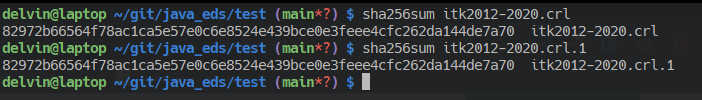
\includegraphics[scale=0.7]{img/some_public_key.png}}
  \caption{Одинаковые хэши файлов}
\end{figure}

По ссылке \url{https://uc-itcom.ru/customers/embeded-cp} можно узнать программу СКЗИ «КриптоПро CSP», которая используется для ЭЦП.

По почте \m{dit@minsvyaz.ru} можно найти документ-инструкцию как установить сертификат ГУЦ (\url{https://moscow.roskazna.gov.ru/upload/iblock/71e/instruktsiya-po-ustanovke-sertifikata-guts-i-novogo-konevogo-sertfiikata-uts-fk.pdf}).

По итогу этой мини исследовательской работы стало известно, что файлы, которые отправляет учебный отдел вуза не являются <<чёрным ящиком>>,
а просто закодированная в определенную структуру ЭЦП с использованием программы СКЗИ <<КриптоПро CSP>>.